\documentclass[final]{beamer}
\usepackage[ngerman]{babel}
\usepackage[utf8]{inputenc}
\usepackage[T1]{fontenc}
\usepackage{lmodern}
\usepackage{listings}
\usepackage{graphicx}
\usepackage{color}
\usepackage{amssymb}

\newcommand{\ThemeFolder}{FSIBeamerTheme}
\RequirePackage{\ThemeFolder/beamerthemeFSI}


\DeclareGraphicsExtensions{.pdf,.png}

\mode<presentation>

\title{Programmiervorkurs für Erstsemester}

\setbeamertemplate{title page}{
  \begin{center}
    \color{FSIblue}
      \resizebox{\textwidth}{!}{Programmiervorkurs}\\
      \vspace{0.3\baselineskip}
      \huge{Einführung in Java}\\
      \huge{Tag 4}
      \vfill
      \large{Daniel Hoff}\\
      \tiny{SS 2013}
  \end{center}
}

\begin{document}

\lstset{tabsize=4}
\lstset{basicstyle=\small}
\lstset{language=java}

\begin{frame}
  \titlepage
\end{frame}

\begin{frame}
  \tableofcontents
\end{frame}

\section{Über mich}
\begin{frame}
	\frametitle{Über mich}
	\textbf{Daniel Hoff}
	\begin{itemize}
		\item{6. Semester Informatik}
		\item{aktiver Fachschafter}
		\item{gewählter studentischer Vertreter im Fakultätsrat}
		\item{Vorsitzender des Fachschaftsvereins}
	\end{itemize}
\end{frame}

\section{Methoden}
\begin{frame}[containsverbatim]
	\frametitle{Beispiel ohne Methoden}
	\begin{lstlisting}
public class Main {
	public static void main() {
		for (int i = 1; i <= 10; i++) {
			System.out.println(i);
		}
		
		// weiterer Code
		
		for (int i = 1; i <= 10; i++) {
			System.out.println(i);
		}
	}
}
	\end{lstlisting}
\end{frame}

\subsection{Warum?}
\begin{frame}
	\frametitle{Warum?}
	\textbf{Probleme?}
	\begin{itemize}
		\item{zeitaufwändig}
		\item{(zu) viel Code}
		\item{unübersichtlich}
		\item{Änderungen kosten noch mehr Zeit}
		\item{Code oft nicht wiederverwendbar}
		\item{Arbeitsteilung kaum möglich}
	\end{itemize}
	\pause
	\vspace{\baselineskip}
	\textbf{Lösungen?}
	\pause
	\begin{itemize}
		\item{ähnlichen Code auslagern}
		\item{wiederverwendbaren Code schreiben}
		\item{\textbf{Methoden!}}
	\end{itemize}
\end{frame}

\begin{frame}[containsverbatim]
	\frametitle{Beispiel mit Methoden}
	\begin{lstlisting}
public class Main {
	public static void main () {
		zaehlBisZehn();
		
		// weiterer Code
		
		zaehlBisZehn();
	}
	
	public static void zaehlBisZehn() {
		for (int i = 1; i <= 10; i++) {
			System.out.println(i);
		}
	}
}
	\end{lstlisting}
\end{frame}

\subsection{Wie?}
\begin{frame}[containsverbatim]
	\frametitle{Kopf der Methode}
	\begin{lstlisting}
public static void zaehlBisZehn () { 
	...
}
	\end{lstlisting}
	\begin{itemize}
		\item{\textbf{public static} immer am Anfang (wird im Vorkurs nicht behandelt)}
		\item{\textbf{Methodenname} vor den runden Klammern}
	\end{itemize}
\end{frame}

\begin{frame}[containsverbatim]
	\frametitle{Aufruf einer Methode}
	\begin{lstlisting}
public static void Main () {
	zaehlBisZehn();
}
	\end{lstlisting}
	\begin{itemize}
		\item{Methodenname}
		\item{()}
		\item{;}
	\end{itemize}
\end{frame}

\subsection{Mehr!}
\begin{frame}
	\frametitle{Methoden können mehr!}
	\begin{itemize}
		\item{Beim Methodenaufruf können zusätzliche Informationen (= Parameter) an die Methode übergeben werden}
		\item{Methoden können Informationen an den Aufrufer zurück geben}
		\item{Methoden können sich selbst aufrufen (= Rekursion) (nicht Teil des Vorkurses)}
	\end{itemize}
\end{frame}

\subsubsection{Methoden mit Parameter}
\begin{frame}[containsverbatim]
	\frametitle{Beispiel ohne Methoden}
	\begin{lstlisting}[escapechar=!]
public class Main () {
	public static void main() {
		for (int i = 1; i <= !\color{red}\textbf{9}!; i++) {
			System.out.println(i);
		}
		
		// weiterer Code
		
		for (int i = 1; i <= !\color{red}\textbf{10}!; i++) {
			System.out.println(i);
		}
	}
}
	\end{lstlisting}
\end{frame}

\begin{frame}[containsverbatim]
	\frametitle{Beispiel mit Methoden}
	\begin{lstlisting}[escapechar=!]
public class Main() {
	public static void main() {
		zaehleBis(!\color{red}\textbf{9}!);
		
		// weiterer Code
		
		zaehleBis(!\color{red}\textbf{10}!);
	}

	public static void zaehleBis(!\textbf{\color{blue}int \color{red}z}!) {
		for (int i = 1; i <= !\color{red}\textbf{z}!; i++) {
			System.out.println(i);
		}
	}
}
	\end{lstlisting}
\end{frame}

\begin{frame}[containsverbatim]
	\frametitle{Kopf der Methode}
	\begin{lstlisting}[escapechar=!]
public static void zaehleBis(!\color{blue}int \color{red}z!) {
	...
}
	\end{lstlisting}
	\begin{itemize}
		\item{In die runden Klammern kommen die Paramter}
		\item{Parameter werden mit Komma getrennt:
			\begin{lstlisting}[escapechar=!]
(!\color{blue}int \color{red}a!, !\color{blue}boolean \color{red}b!, !\color{blue}double \color{red}c!)
			\end{lstlisting}
		}
		\item{Ein Parameter besteht aus {\color{blue}Datentyp} und \color{red}Bezeichner}
	\end{itemize}
\end{frame}

\begin{frame}[containsverbatim]
	\frametitle{Aufruf}
	\begin{lstlisting}[escapechar=!]
pulic static void main() {
	zaehleBis(!\color{red}9!);
	zaehleBis(!\color{red}10!);
}
	\end{lstlisting}
	\begin{itemize}
		\item{Parameter, die man übergeben möchte, durch Komma getrennt in die Runden Klammern}
	\end{itemize}
\end{frame}

\begin{frame}[containsverbatim]
	\frametitle{Was passiert?}
	\begin{itemize}
		\item{
			\begin{lstlisting}[escapechar=!]
zaehleBis(!\color{red}9!);
			!\vspace{\baselineskip}!
public static void zaehleBis(!\color{blue}int \color{red}z!) {
	// z wird der Wert 9 zugewiesen
}
			\end{lstlisting}
		}
		\vspace{\baselineskip}
		\item{
			\begin{lstlisting}[escapechar=!]
zaehleBis(!\color{red}10!);
			!\vspace{\baselineskip}!
public static void zaehleBis(!\color{blue}int \color{red}z!) {
	// z wird der Wert 10 zugewiesen
}
			\end{lstlisting}
		}
	\end{itemize}
\end{frame}

\begin{frame}[containsverbatim]
	\frametitle{Beispiel mit 2 Parametern}
	\begin{lstlisting}[escapechar=!]
public class Main {
	public static void main() {
		zaehleVonBis(!\color{blue}1!, !\color{red}9!);
		// weiterer Code
		zaehleVonBis(!\color{blue}5!, !\color{red}10!);
	}
	
	public static void 
		zaehleVonBis(int !\color{blue}v!, int !\color{red}b!) {
		for (int i = !\color{blue}v!; i <= !\color{red}b!; i++) {
			System.out.println(i);
		}
	}
}
	\end{lstlisting}
\end{frame}

\subsubsection{Methoden mit Rückgabewert}
\begin{frame}[containsverbatim]
	\frametitle{Beispiel mit Rückgabewert}
	\begin{lstlisting}[escapechar=!]
public class Main {
	public static void main() {
		!\color{blue}int! !\color{red}x! = zaehleVonBis(1, 9);
	}
	
	public static !\color{blue}int! 
		zaehleVonBis(int v, int b) {
		for (int i = v; i <= b; i++) {
			System.out.println(i);
		}
		
		!\color{blue}return! !\color{red}b - v + 1!;
	}
}
	\end{lstlisting}
\end{frame}

\begin{frame}[containsverbatim]
	\frametitle{Kopf der Methode}
	\begin{lstlisting}[escapechar=!]
public static !\color{blue}int! zaehleVonBis(int v, int b) {
	...
	!\color{blue}return! !\color{red}b - v + 1!;
}
	\end{lstlisting}
	\begin{itemize}
		\item{Möchte man keinen Wert zurück geben, so kommt nach \textbf{static} das Schlüsselwort \color{blue}void}
		\item{Ansonsten wird {\color{blue}void} durch den gewünschten Datentyp ersetzt}
		\item{Mit {\color{blue}return} wird der Wert zurückgegeben. Das {\color{blue}return} ist Pflicht und muss erreicht werden}
	\end{itemize}
\end{frame}

\begin{frame}[containsverbatim]
	\frametitle{Was passiert?}
	\begin{lstlisting}[escapechar=!]
!\color{blue}int! !\color{red}x! = zaehleVonBis(1, 9);
	\end{lstlisting}
	\begin{itemize}
		\item{Rechte Seite von "\textbf{=}"\ wird zuerst ausgewertet
			\begin{itemize}
				\item{zaehleVonBis(1, 9);}
			\end{itemize}
		}
	\end{itemize}
	\begin{lstlisting}[escapechar=!]
public static !\color{blue}int! zaehleVonBis(int v, int b) {
	...
	!\color{blue}return! !\color{red}b - v + 1!;
}
	\end{lstlisting}
	\begin{itemize}
		\item{v = 1, b = 9
			\begin{itemize}
				\item{return 9 - 1 + 1 = 9}
					\begin{itemize}
						\item{9 wird zurückgegeben}
					\end{itemize}
			\end{itemize}
		}
		\item{{\color{red}x} wird der Wert 9 zugewiesen}
	\end{itemize}
\end{frame}

\begin{frame}[containsverbatim]
	\frametitle{Generell}
	\begin{lstlisting}[escapechar=!]
public static !\color{blue}Rückgabetyp! !\color{green}Name! (!\color{red}Parameter!) {
	// Methodenrumpf
	!\color{blue}return! ... ; 
}
	\end{lstlisting}
	\begin{itemize}
		\item{Wenn der {\color{blue}Rückgabetyp} \textbf{void} ist, darf kein {\color{blue}return} vorkommen}
	\end{itemize}
\end{frame}

\section{Klassenvariablen}
\begin{frame}[containsverbatim]
	\frametitle{Beispiel ohne Klassenvariablen}
	\begin{lstlisting}[escapechar=!]
public class Main {
	public static void main() {
		!\color{blue}int! !\color{red}x! = zaehleVonBis(1, 9);
	}
	
	public static !\color{blue}int! 
		zaehleVonBis(int v, int b) {
		for (int i = v; i <= b; i++) {
			System.out.println(i);
		}
		
		boolean wurdeAusgegeben = b >= v;
		
		!\color{blue}return! !\color{red}b - v + 1!;
	}
}
	\end{lstlisting}
\end{frame}

\subsection{Warum?}
\begin{frame}
	\frametitle{Warum?}
	\textbf{Probleme}
	\begin{itemize}
		\item{Methoden können nur einen Wert zurückgeben}
		\item{Eine Methode kann nicht auf Daten aus anderen Methoden zugreifen}
	\end{itemize}
	\vspace{\baselineskip}
	\pause
	\textbf{Lösungen}
	\pause
	\begin{itemize}
		\item{\textbf{Klassenvariablen}
			\begin{itemize}
				\item{mit Bedacht verwenden!}
			\end{itemize}
		}
	\end{itemize}
\end{frame}
	
\subsection{Wie?}
\begin{frame}[containsverbatim]
	\frametitle{Beispiel mit Klassenvariablen}
	\begin{lstlisting}[escapechar=!]
public class Main {
	!\color{blue}public static boolean! !\color{red}wurdeAusgegeben!;
	public static void main() {
		int x = zaehleVonBis(1, 9);
		System.out.println(wurdeAusgegeben);
	}
	
	public static int 
		zaehleVonBis(int v, int b) {
		for (int i = v; i <= b; i++) {
			System.out.println(i);
		}
		!\color{red}wurdeAusgegeben! = b >= v;
		return b - v + 1;
	}
}
	\end{lstlisting}
\end{frame}

\begin{frame}[containsverbatim]
	\frametitle{Deklaration von Klassenvariablen}
	\begin{itemize}
		\item{Deklaration direkt nach Klassendeklaration}
		\item{\textbf{public static} {\color{blue}Datentyp} {\color{red}Bezeichner};}
		\item{sichtbar in der ganzen Klasse}
		\item{Ohne manuelle Zuweisung wird der Defaultwert zugewiesen}
		\item{Beispiel:
			\begin{lstlisting}[escapechar=!]
public static !\color{blue}boolean! !\color{red}wurdeAusgegeben!;
			\end{lstlisting}
		}
	\end{itemize}
\end{frame}

\section{Aufgabe}
\begin{frame}
	\frametitle{Vorstellung der Aufgabe}
	\begin{columns}[T]
		\column{0.5\textwidth}
			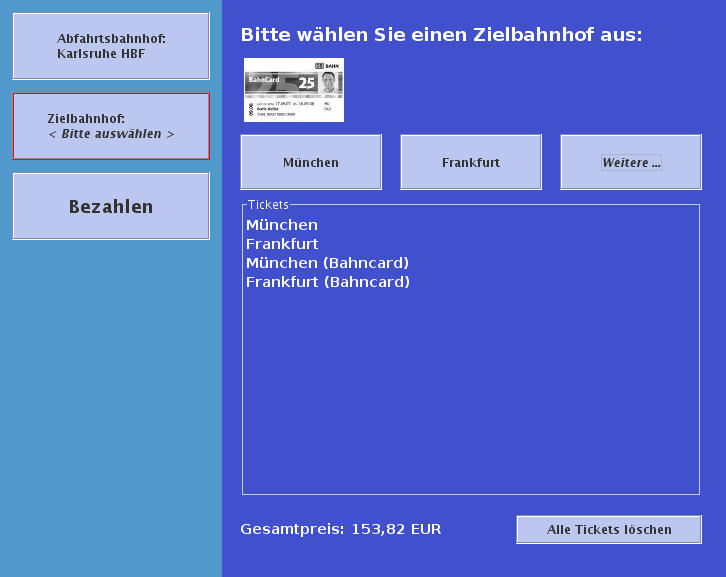
\includegraphics[width=\textwidth]{gfx/bahnticketautomat_buchen}
		\column{0.5\textwidth}
			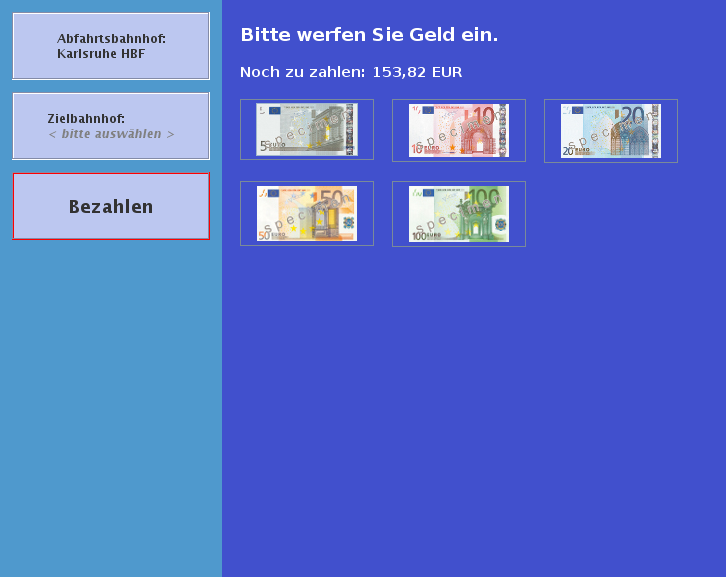
\includegraphics[width=\textwidth]{gfx/bahnticketautomat_bezahlen}
	\end{columns}
	\vspace{\baselineskip}
	\begin{columns}[T]
		\column{0.5\textwidth}
			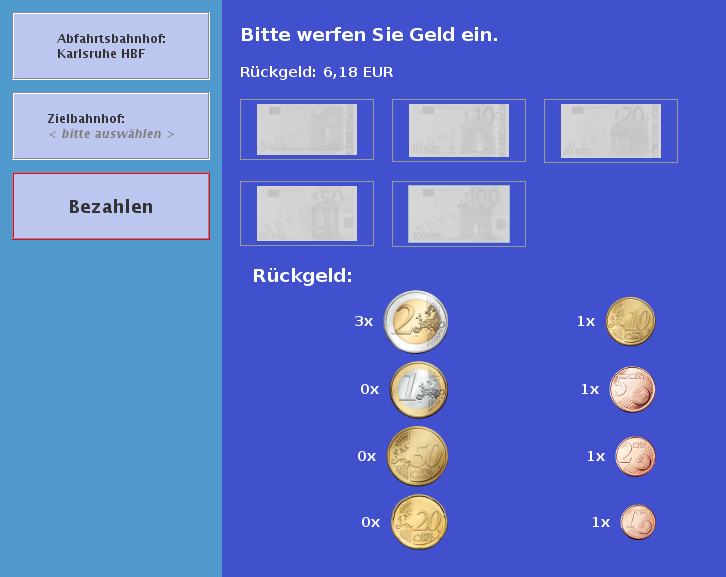
\includegraphics[width=\textwidth]{gfx/bahnticketautomat_rueckgeld}
		\column{0.5\textwidth}
		\pause
			
\includegraphics[width=\textwidth]{gfx/Wait-what-meme-rage-face.jpg}
	\end{columns}
	
\end{frame}

\section{Quellen \& Lizenz}
\begin{frame}
	\frametitle{Quellen und Lizenz}
	\begin{center}
		
\includegraphics[width=250px]{gfx/fsi}
	\end{center}
	\begin{itemize}
		\item{Original von Samuel Zeitvogel}
		\item{Überarbeitet 2012 von Daniel Hoff}
	\end{itemize}
\end{frame}

\end{document}
